\documentclass{article}

\usepackage[utf8]{inputenc} % allow utf-8 input
\usepackage{amsmath}
\usepackage{graphicx}
\usepackage{epsfig}
\usepackage[tight]{subfigure}

% 1-inch margins, from fullpage.sty by H.Partl, Version 2, Dec. 15, 1988.
\topmargin 0pt
\advance \topmargin by -\headheight
\advance \topmargin by -\headsep
\textheight 8.9in
\oddsidemargin 0pt
\evensidemargin \oddsidemargin
\marginparwidth 0.5in
\textwidth 6.5in

\parindent 0in

\newcommand{\newfig}[7]{
\begin{figure}[h!] 
\centering
\begin{subfigure}[#1.jpg]
{
\includegraphics[width=0.23\textwidth]{figures/result/#1/#1}
\includegraphics[width=0.23\textwidth]{figures/result/#1/#1-llel}
\includegraphics[width=0.23\textwidth]{figures/result/#1/#1-perp}
\includegraphics[width=0.23\textwidth]{figures/result/#1/#1-rectified}
}
\end{subfigure}
\label{fig:#1}
\end{figure}


\subsubsection{Figure: #1.jpg}

& &

}



\title{16822 - Geometry based vision - Homework 1}

\author{
  Michael Jaison Gnanasekar\\
  Andrew Id: mgnanase\\
  Robotics Institute\\
  Carnegie Mellon University\\
  Pittsburgh, PA 15213 \\
  \texttt{mgnanase@andrew.cmu.edu} \\
 }

\begin{document}

\maketitle

\section{Problem 1}

\subsection{H for mirror reflection image}

\subsubsection{}
Let a point in world as $P$ and its reflection around $L$ as $P'$. Also, let $R$ be the rotation that defines the reflection around the line $L$. ie. $P' = RP$

\begin{align*}
p &= K [ I | 0 ] P \\
p' &= K [ I | 0 ] P' \\
&= K [ I | 0 ] RP \\
&= K [ I | 0 ] R K^{-1} p \\
p' &= K R K^{-1} p \\
\end{align*}

Hence the homography exist as $H = K R K^{-1}$.

\subsubsection{}
\begin{align*}
H^2 &= (K R K^{-1}) (K R K^{-1}) \\
&= I
\end{align*}
Since $R$ is orthogonal matrix, $H^2 = I$.


\subsection{Fun with pencils of line}

\subsubsection{}
Slope of the line: $\frac{-u}{v}$

\subsubsection{}
Any lines in the pencil of lines can be represented as a linear combination of two lines. Since we are dealing with projective 1-D space.

\subsubsection{}
Dimension of H is 2x2. Since the projective space is 1D.

\subsubsection{}
\begin{align*}
H = \begin{pmatrix}
h_1 & h_2 & 0 \\
h_3 & h_4 & 0 \\
0 & 0 & 1
\end{pmatrix}
\end{align*}

By homography,
\begin{align*}
l' &= H \begin{pmatrix} u \\ v \\ w \end{pmatrix} \\
l' &= \begin{pmatrix} h_1 & h_2 & 0 \\ h_3 & h_4 & 0 \\ 0 & 0 & 1 \end{pmatrix} \begin{pmatrix} u \\ v \\ w \end{pmatrix} \\
&= \begin{pmatrix} h_1 u + h_2 v \\ h_3 u + h_4 v \\ w \end{pmatrix} \\
\end{align*}

The slope is given by $\frac{-u}{v}$. \\
\begin{align*}
s' &= - \frac{h_1 u + h_2 v}{h_3 u + h_4 v} \\
&= - \frac{h_1 \frac{u}{v} + h_2 }{h_3 \frac{u}{v} + h_4 } \\
\end{align*}

Hence, it can be expressed in terms of slope $s$.
\begin{align*}
s' &=  \frac{h_1 s + h_2 }{h_3 s + h_4 } \\
\end{align*}


\subsubsection{}
The determinant of the matrix H should not be zero. The homography should be invertible. So, $ad - bc \neq 0$


\subsection{Rodrigues’s rotation formula (and some motion)}

\subsubsection{Matrix notation}

\begin{align*}
R &= I + sin(\theta) [w]_x  + (1 - cos(\theta)) [w]_x^2 \\
[w]_x = W &= 
\begin{pmatrix}
0 & -w_3 & w_2 \\
w_3 & 0 & -w_1 \\
-w_2 & w_1 & 0 \\
\end{pmatrix}
\end{align*}

\subsubsection{}

When $\theta$ is small, $sin(\theta)$ tends to $\theta$, $cos(\theta)$ tends to $1 - \frac{\theta^2}{2}$. Hence, $Rp$ is:

\begin{align*}
Rp &= I p + \theta W p + \frac{\theta^2}{2} W^2 p \\
&= I p + [\omega]_x p + \frac{[\omega]_x^2}{2}  p \\
&= I p + \Omega p + \frac{\Omega^2}{2} p \\
\end{align*}


\subsubsection{}
Essestial matrix is given by,

\begin{align*}
E &= [t]_x R \\
&= [t]_x ( I + \Omega + \frac{\Omega^2}{2} ) \\
\end{align*}


\subsubsection{}
Epipole in one image is $t$.  $i.e.$ $e' = t$. \\

Epipole in other image is given by, $e = K R^T t$. Since $K = I$,
\begin{align*}
e &= R^T t \\
&= ( I + \Omega + \frac{\Omega^2}{2} )^T t \\
&= I^T t + \Omega^T t + \frac{(\Omega^2)^T}{2}  t  \\
\end{align*}
(since $\Omega$ is skew symmetric, $\Omega^T = - \Omega$) \\
\begin{align*}
e &= I t - \Omega t + \frac{(\Omega^2)^T}{2} t  \\
\end{align*}
Also, since the translation vector $t$ is parallel to rotation axis $w$, $w \times t = 0$. Hence,
\begin{align*}
e &= t  \\
\end{align*}


\subsubsection{}
Projection of $[X\ Y\ Z\ 1]^T$ in Camera-1 is $[u\ v\ 1]^T$. Similarly, projection in Camera-2 is given by $[u'\ v'\ 1]^T$.

\begin{align*}
\begin{pmatrix} u\\ v\\ 1 \end{pmatrix} &= K [I | 0] \begin{pmatrix} X\\ Y\\ Z\\ 1 \end{pmatrix} \\
Since\ K = I \\
\begin{pmatrix} u\\ v\\ 1 \end{pmatrix} &= \begin{pmatrix} X/Z\\ Y/Z\\ 1 \end{pmatrix} \\
\end{align*}
Similarly,
\begin{align*}
\begin{pmatrix} u'\\ v'\\ 1 \end{pmatrix} &=  [R | t] \begin{pmatrix} X\\ Y\\ Z\\ 1 \end{pmatrix} \\
\end{align*}

From the equation $9.7$ from \cite{1} Multiple View Geometry in Computer Vision book by Zisserman, the mapping from an image point $p$ to an image point $p'$ is given by
\begin{align*}
p' &= K' R K^{-1} p + K' t/Z \\
(since\ K = K' = I) \\
p' &= R p + t/Z \\
\begin{pmatrix} u'\\ v'\\ 1 \end{pmatrix} &= ( I + \Omega + \frac{\Omega^2}{2} ) \begin{pmatrix} u\\ v\\ 1 \end{pmatrix} + t / Z \\
\begin{pmatrix} u + du\\ v + dv\\ 1 \end{pmatrix} &= \begin{pmatrix} u\\ v\\ 1 \end{pmatrix} + ( \Omega + \frac{\Omega^2}{2} ) \begin{pmatrix} u\\ v\\ 1 \end{pmatrix} + t / Z \\
\begin{pmatrix} du\\  dv\\ 1 \end{pmatrix} &= ( \Omega + \frac{\Omega^2}{2} ) \begin{pmatrix} u\\ v\\ 1 \end{pmatrix} + t / Z \\
\end{align*}
From above equation, $du$ and $dv$ are expressed as a function of $u$, $v$, $\Omega$, $t$, and $Z$.


\subsubsection{}
Scene plane homography is defined as
\begin{align*}
H &= R - \frac{t n^T}{d}
\end{align*}
Since the point $P$ is on a plane $(n, d)$, the point in camera-2 $p'$ is defined as
\begin{align*}
p' &= H p \\
\begin{pmatrix} u'\\ v'\\ 1 \end{pmatrix} &= H \begin{pmatrix} u\\ v\\ 1 \end{pmatrix} \\
&= (R - \frac{t n^T}{d}) \begin{pmatrix} u\\ v\\ 1 \end{pmatrix} \\
&= (I + \Omega + \frac{\Omega^2}{2} - \frac{t n^T}{d}) \begin{pmatrix} u\\ v\\ 1 \end{pmatrix} \\
\begin{pmatrix} u + du\\ v + dv\\ 1 \end{pmatrix} &= \begin{pmatrix} u\\ v\\ 1 \end{pmatrix} + (\Omega + \frac{\Omega^2}{2} - \frac{t n^T}{d}) \begin{pmatrix} u\\ v\\ 1 \end{pmatrix} \\
\begin{pmatrix} du\\  dv\\ 1 \end{pmatrix} &= (\Omega + \frac{\Omega^2}{2} - \frac{t n^T}{d}) \begin{pmatrix} u\\ v\\ 1 \end{pmatrix} \\
\end{align*}
From the above equation, it is shown that $du$ and $dv$ does not depend on the depth $Z$.


\subsubsection{}
The expression of $du$ and $dv$ is given by,
\begin{align*}
\begin{pmatrix} du\\  dv\\ 1 \end{pmatrix} &= (\Omega + \frac{\Omega^2}{2} - \frac{t n^T}{d}) \begin{pmatrix} u\\ v\\ 1 \end{pmatrix} \\
\end{align*}


\subsubsection{}
Scene plane homography is defined as
\begin{align*}
H &= R - \frac{t n^T}{d} \\
&= I + \Omega + \frac{\Omega^2}{2} - \frac{t n^T}{d} \\
\end{align*}


\subsubsection{}
Since the robot is moving on ground plane, $\Omega$ and $t$ is orthogonal to $n$. \\
To find the point that is invariant to $H$, we need to find the point for which $H$ is $I$. \\
Assuming that $H$ is $I$,
\begin{align*}
I = I + \Omega + \frac{\Omega^2}{2} - \frac{t n^T}{d} \\
\Omega + \frac{\Omega^2}{2} - \frac{t n^T}{d} = 0
\end{align*}
From the above equation, it is clear that we are interested in the null space of the above matrix. \\
The rank of last term $\frac{t n^T}{d}$ is 1, and $t$ is in the null space of $t n^T$. \\
And since we have proved $e = t$, the point that is invariant to $H$ is $e$. The epipole.


\section{Problem 2}

Image rectification is split into two sub problems.
\begin{itemize}
    \item Affine Rectification
    \item Euclidean Rectification
\end{itemize}

\subsection{Affine Rectification}
Algorithm.
\begin{itemize}
    \item In the input image, two pairs of parallel lines are annotated.
    \item Find the intersection of parallel lines at point at $\infty$ ($p_{\infty}$).
    \item Find the line at $\infty$ ($L_{\infty}$) connecting two points at $\infty$ as shown in Figure \ref{fig:line_inf}. $L_\infty = [l_1\ l_2\ l_3]^T$.
    \item Create the Homography as 
    \begin{align*}
    H = \begin{pmatrix} 0 & 0 & 0 \\ 0 & 0 & 0 \\ l_1 & l_2 & l_3 \end{pmatrix}
    \end{align*}
    \item Apply warping to the image by the homography $H$.
\end{itemize}

\subsection{Euclidean Rectification}
Algorithm:
\begin{itemize}
    \item Annotate two perpendicular lines in the affine transformed image from the previous section as shown in \ref{fig:line_inf}
    \item Form the below equation, we should solve for the unknowns.
    \begin{align*}
    l_1^T H^{-1} C^* H^{-T} l_2 &= 0 \\
    \end{align*}
    \item As shown in the class, it can be solved by combining $L = AA^T$ and solving $L$.
    \item $L$ can be solved by $L = UDU^T$, where $U^{-1} = U^T$. Because $L$ is symmetric.
    \item Now, the original matrix $A$ can be obtained by $A = U\sqrt{D}U^T$.
    \item From this, the homography matrix $H$ can be framed as 
    \begin{align*}
    H = \begin{pmatrix} AA^T & 0  \\ 0 & 0 \end{pmatrix}
    \end{align*}
\end{itemize}

\subsection{Problems Encountered}

\begin{itemize}
    \item Since the transformation depends on the parallel and perpendicular lines annotation, even a small error in the annotation gave a wrong transformation.
    \item While choosing the perpendicular lines, if the two pairs of perpendicular lines are in the same direction, the system did not solve.
    \item Numerical issues were handled smoothly if the annotation on image is precise.
\end{itemize}



\begin{figure}[h!] 
\centering
\begin{subfigure}[Visualization of Line at $\infty$]
{
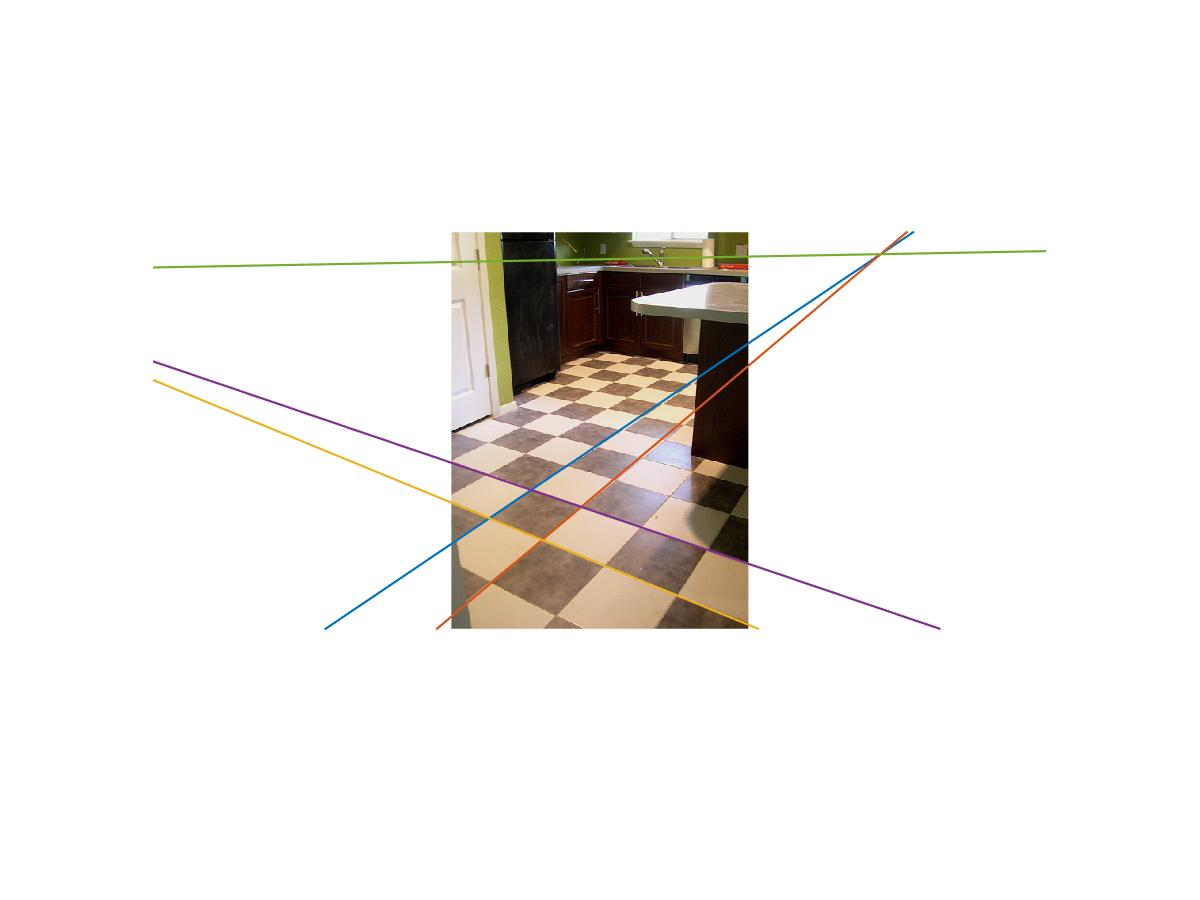
\includegraphics[width=0.45\textwidth]{figures/checker2-llel}
}
\end{subfigure}
\begin{subfigure}[Annotated perpendicular lines]
{
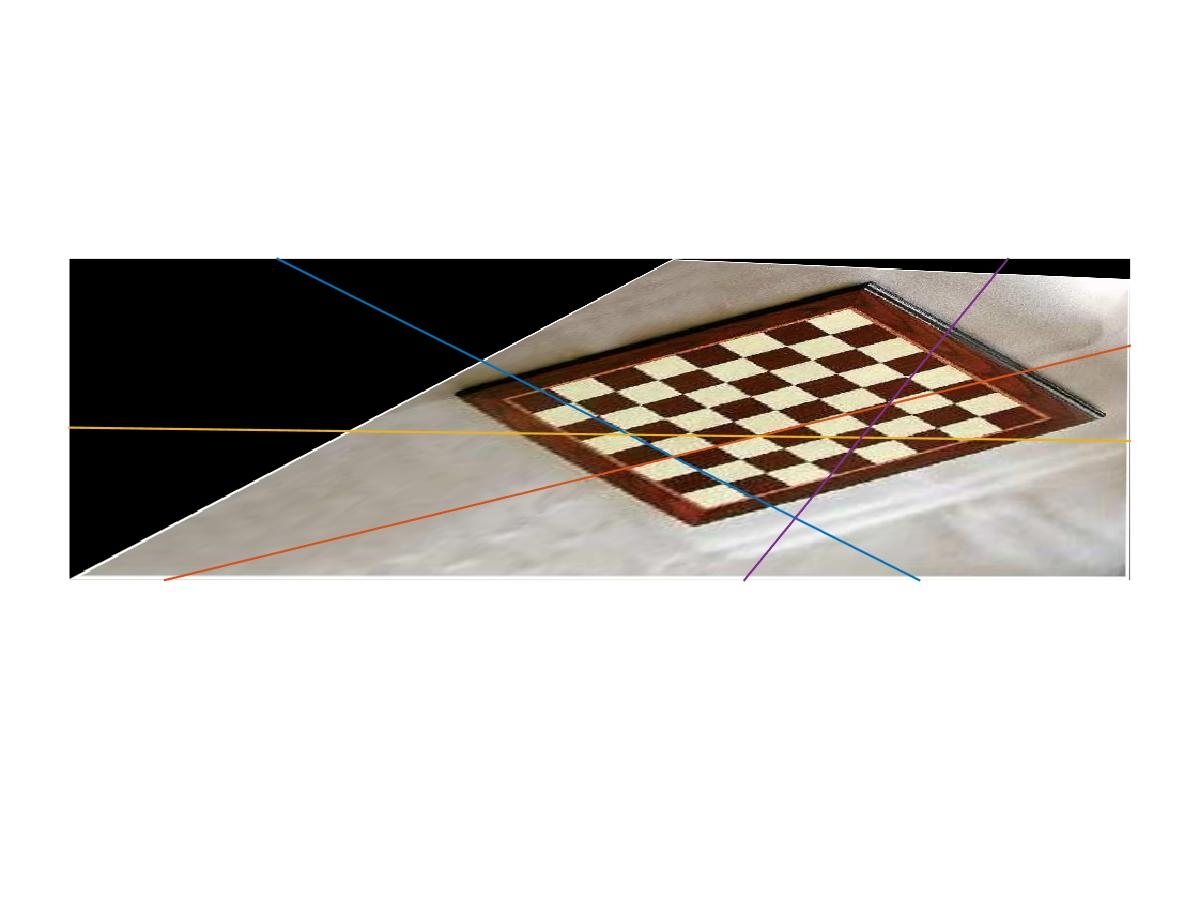
\includegraphics[width=0.45\textwidth]{figures/chess1-perp}
}
\end{subfigure}
\caption{An example of images in the pipeline}
\label{fig:line_inf}
\end{figure}

\subsection{Angles}

\newfig{chess1}{0.7638856}{0}{-0.6249080}{-1.1259619E-16}{-0.5341788}{1.7515324E-01}
\newfig{facade}{0.0246178}{-4.0250391E-16}{0.8654985}{-1.9446465E-16}{-0.2569672}{-1.1198973E-01}
\newfig{tiles3}{-0.3762770}{7.8206839E-17}{0.6189759}{1.0455350E-16}{0.6045568}{-3.5030400E-02}
\newfig{tiles4}{0.3704599}{2.7226264E-16}{0.3541860}{2.3781163E-16}{-0.3501436}{1.5342336E-03}
\newfig{tiles5}{0.2050029}{-1.0660826E-16}{-0.0816590}{0.0000000E+00}{0.2108932}{5.4974449E-03}
\newfig{tiles6}{-0.0258799}{-1.5895978E-16}{-0.0676860}{-6.9942619E-16}{0.0794271}{8.8854489E-03}
\newfig{checker1}{-0.7961622}{4.1091966E-17}{0.9169904}{-2.7865405E-16}{-0.7672571}{1.2124164E-01}

\subsection{Own Images}
\newfig{web-house}{-0.2038131}{-3.6498809E-17}{-0.2921571}{-4.2676765E-16}{-0.1917144}{2.7471455E-02}
\newfig{web2}{-0.5004252}{7.8058757E-17}{0.4175002}{0.0000000E+00}{0.4084644}{8.2416027E-02}
\newfig{web-house2}{0.3003940}{-1.2550527E-16}{-0.4394226}{-8.6467521E-17}{0.3325585}{8.2952982E-02}


\end{document}